\documentclass[fleqn,11pt]{article}

\usepackage[letterpaper,margin=0.75in]{geometry}

\usepackage{amsmath}
\usepackage{booktabs}
\usepackage{graphicx}
\usepackage{listings}
\usepackage{tikz}

\setlength{\parindent}{1.4em}

\begin{document}

\lstset{
  language=Python,
  basicstyle=\small,          % print whole listing small
  keywordstyle=\bfseries,
  identifierstyle=,           % nothing happens
  commentstyle=,              % white comments
  stringstyle=\ttfamily,      % typewriter type for strings
  showstringspaces=false,     % no special string spaces
  numbers=left,
  numberstyle=\tiny,
  numbersep=5pt,
  frame=tb,
}

\title{Lab 1 Report}

\author{Martin Sanchez and Ben Jacobson}

\date{2/1/17}

\maketitle

\section{Two Nodes}

In this first section we explored a simple network consisting of two nodes and one bidirectional link. We simulated the following scenarios:
\begin{enumerate}

\item Set the bandwidth of the links to 1 Mbps, with a propagation delay of 1 second. Send one packet with 1000 bytes from n1 to n2 at time 0.

\item Set the bandwidth of the links to 100 bps, with a propagation delay of 10 ms. Send one packet witih 1000 bytes from n1 to n2 at time 0.

\item Set the bandwidth of the links to 1 Mbps, with a propagation delay of 10 ms. Send three packets from n1 to n2 at time 0 seconds, then one packet at time 2 seconds. All packets should have 1000 bytes.

\end{enumerate}
After running the simulations we will show our network configuration, the output of the simulation and the calculations we used to verify that the output was correct. 

The results of running the simulator for each of the scenarios are below:

\begin{enumerate}
  \item 
    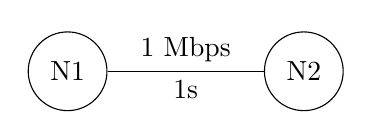
\begin{tikzpicture}
    \node[circle,draw, minimum size=1cm] (A) at (0,0) {N1};
    \node[circle,draw, minimum size=1cm] (B) at (3,0) {N2};
    \draw (A) -- (B) node[pos=0.5, above] {1 Mbps} node[pos=0.5, below] {1s} ; 
    \end{tikzpicture}

    The output of the simulation was:
    \begin{lstlisting} 
    Created:0  ID:1 Received: 1.008
    \end{lstlisting}

    These are our verifying calculations:
    \begin{align*}
    d &= d_{trans} + d_{prop}\\
      &= (1000*8)/1000000 + 1\\
      &= 1.008
    \end{align*}


  \item 
    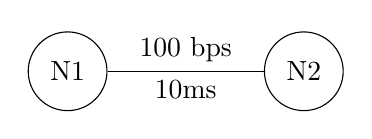
\begin{tikzpicture}
    \node[circle,draw, minimum size=1cm] (A) at (0,0) {N1};
    \node[circle,draw, minimum size=1cm] (B) at (3,0) {N2};
    \draw (A) -- (B) node[pos=0.5, sloped, above] {100 bps} node[pos=0.5, sloped, below] {10ms};
    \end{tikzpicture}

    The output of the simulation was: 
    \begin{lstlisting}
      Created:0  ID:1 Received: 80.01
    \end{lstlisting}

    These are our verifying calculations:
    \begin{align*}
    d &= d_{trans} + d_{prop}\\
      &= (1000*8)/100 + 0.01\\
      &= 80.01
    \end{align*}
  \item 
    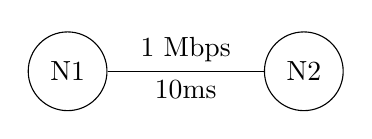
\begin{tikzpicture}
    \node[circle,draw, minimum size=1cm] (A) at (0,0) {N1};
    \node[circle,draw, minimum size=1cm] (B) at (3,0) {N2};
    \draw (A) -- (B) node[pos=0.5, sloped, above] {1 Mbps} node[pos=0.5, sloped, below] {10ms};
    \end{tikzpicture}

  The output of the simulation was:
  \begin{lstlisting}
    Created:0  ID:1  Received:0.018000000000000002
    Created:0  ID:2  Received:0.026000000000000002
    Created:0  ID:3  Received:0.034
    Created:2.0  ID:4  Received:2.018
  \end{lstlisting}
  These are our verifying calculations:
  \begin{align*}
    d1 &= d1_{trans} + d1_{prop}\\
      &= (1000*8)/1000000 + 0.01\\
      &= 0.018
  \end{align*}
  \begin{align*}
    d2 &= d1_{trans} + d2_{trans} + d2_{prop} \\
      &= 0.018 + (1000*8)/1000000 + 0.01\\
      &= 0.026
  \end{align*}
  \begin{align*}
    d3 &= d2_{trans} + d3_{trans} + d3_{prop}\\
      &= 0.026 + (1000*8)/1000000 + 0.01\\
      &= 0.034
  \end{align*}
  \begin{align*}
    d4 &= 2.0 + d4_{trans} + d4_{prop}\\
      &= 2.0 + (1000*8)/1000000 + 0.01\\
      &= 2.018
  \end{align*}
  
\end{enumerate}

\section{Three Nodes}

In this section we will use the simulator to setup a network consisting of three nodes and two links. We will test two fast links and one fast link with a slow link. For each scenario we will show our network configuration, the last 5 lines of the simulation ouput and the calculations we used to verify the output.
The results are as follows:  

\begin{enumerate}
  \item 
  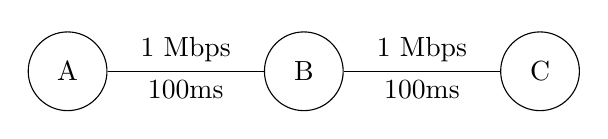
\begin{tikzpicture}
    \node[circle,draw, minimum size=1cm] (A) at (0,0) {A};
    \node[circle,draw, minimum size=1cm] (B) at (3,0) {B};
    \node[circle,draw, minimum size=1cm] (C) at (6,0) {C};
    \draw (A) -- node[pos=0.5,above] {1 Mbps} node[midway,below]{100ms}(B) -- (C) node[pos=0.5,above] {1 Mbps} node[midway,below]{100ms};
  \end{tikzpicture}

  Our data for the two fast links is below:
  \begin{lstlisting}
    1Mbps
    Created:0  ID:995  Received:8.176000000000007
    Created:0  ID:996  Received:8.184000000000006
    Created:0  ID:997  Received:8.192000000000007
    Created:0  ID:998  Received:8.200000000000006
    Created:0  ID:999  Received:8.208000000000007

    1Gbps
    Created:0  ID:995  Received:0.2079760000000001
    Created:0  ID:996  Received:0.2079840000000001
    Created:0  ID:997  Received:0.20799200000000012
    Created:0  ID:998  Received:0.20800000000000013
    Created:0  ID:999  Received:0.20800800000000014
  \end{lstlisting}
  After examining our output we determined that the transmission delay dominated.
  \newline
  These are our verifying calculations:
  \begin{align*}
    d &= d_{trans1} + d_{prop1} + (1000 * d_{trans2}) + d_{prop2}\\
      &= ((1000*8)/1000000) + .1 + (1000 * (1000*8)/1000000) + 0.1\\
      &= 0.008 + 0.1 + (1000 * 0.008) + 0.1\\
      &= 8.208
  \end{align*}
  \begin{align*}
    d &= d_{trans1} + d_{prop1} + (1000 * d_{trans2}) + d_{prop2}\\
      &= ((1000*8)/1000000000) + .1 + (1000 * (1000*8)/1000000000) + 0.1\\
      &= 0.000008 + 0.1 + (1000 * 0.000008) + 0.1\\
      &= 0.208008
  \end{align*}

  \item 
  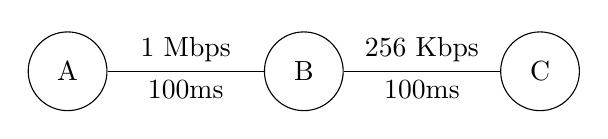
\begin{tikzpicture}
    \node[circle,draw, minimum size=1cm] (A) at (0,0) {A};
    \node[circle,draw, minimum size=1cm] (B) at (3,0) {B};
    \node[circle,draw, minimum size=1cm] (C) at (6,0) {C};
    \draw (A) -- node[pos=0.5,above] {1 Mbps}  node[midway,below]{100ms}(B) -- (C) node[pos=0.5, above] {256 Kbps}  node[midway,below]{100ms};
  \end{tikzpicture}

  Our data for the one fast link and one slow link is below: 
  \begin{lstlisting}
    Created:0  ID:995  Received:31.333000000000002
    Created:0  ID:996  Received:31.364250000000002
    Created:0  ID:997  Received:31.395500000000002
    Created:0  ID:998  Received:31.426750000000002
    Created:0  ID:999  Received:31.458000000000002
  \end{lstlisting}
  These are our verifying calculations:
  \begin{align*}
    d &= d_{trans1} + d_{prop1} + (1000 * d_{trans2}) + d_{prop2}\\
      &= ((1000*8)/1000000) + .1 + (1000 * (256*8)/1000000) + 0.1\\
      &= 0.008 + 0.1 + (1000 * 0.03125) + 0.1\\
      &= 31.458
  \end{align*}

\end{enumerate}

% \vspace{0.5cm}
% \begin{tabular}{lc}
%   \toprule
%   Setting & Result\\
%   \midrule
%   1 & 1.0\\
%   2 & 3.45\\
%   3 & 7.85\\
%   4 & 15.89\\
%   \bottomrule
% \end{tabular}
% \vspace{0.5cm}


\section{Queueing Theory}
In this section we explore whether or not the simulator can validate basic queueing theory. 
We use the same configuration as the twonodes3.txt. 
\newline
\newline
The node configuration is shown below:
\newline

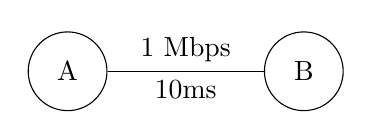
\begin{tikzpicture}
    \node[circle,draw, minimum size=1cm] (A) at (0,0) {A};
    \node[circle,draw, minimum size=1cm] (B) at (3,0) {B};
    \draw (A) -- (B) node[pos=0.5, sloped, above] {1 Mbps} node[pos=0.5, sloped, below] {10ms};
\end{tikzpicture}

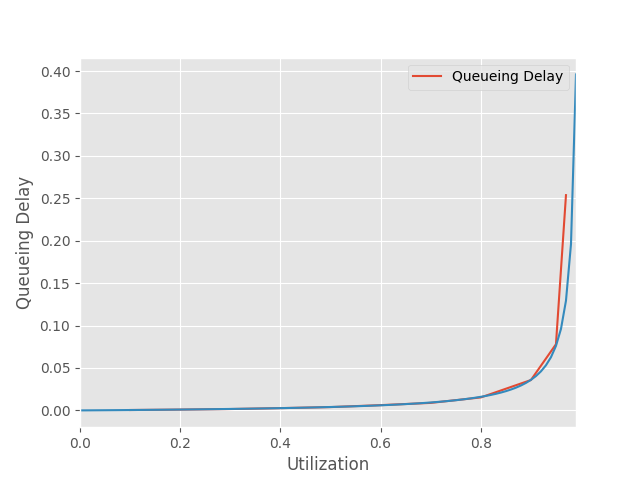
\includegraphics[width=11cm]{graphs/line}
\newline
This is the graph of our queue theory output. As you can see the red is the experimental queueing delay data. The Blue line is the theoretical data. It is apparent that the simulator does indeed validate basic queueing theory. However, like any experimental model the simulator is inperfect and there are slight differences above the 80\% usage mark.
\newline
\newline
The load we used to generate cover the full range of values from 0 to 1. We used extra points in the range from 0.9 to 1.0 to get more data points in this critical range. The data is found in the following table:
\begin{center}
  \begin{tabular}{c c}
  \hline
  Rate & Load \\ [0.5ex]
  \hline\hline
  0.1 & 12.5 \\
  0.2 & 25.0 \\
  0.3 & 37.5 \\
  0.4 & 50.0 \\
  0.5 & 62.5 \\
  0.6 & 75.0 \\
  0.7 & 87.5 \\
  0.8 & 100.0 \\
  0.9 & 112.5 \\
  0.95 & 118.75 \\
  0.97 & 121.25 \\ [1ex]
  \end{tabular}
  \end{center}

The data we collected follows the theoretical exponential curve proving that the bene simulator can correctly simulate queueing theory. 
\section{Summary}
In this lab we successfully explored some of the basic functionality of the bene simulator. We were able to simulate a two node basic network with various bandwidths and propagation delays. We then even sent multiple packets of data across our networks and the simulator responded well. See section on two nodes. 
\newline
\newline
In the section on three nodes, we explored a slightly more complicated network consisting of three nodes and two links. The first scenario contained two links with the same exact bandwidth and propagation delay. While the second scenario included a link that was about 75\% of the speed as the first link. The simulator also responded well to and gave us the same answers as we got in our calulations by hand. See section on three nodes.
\newline
Lastly, we were able to prove that the Bene simulator can correctly validate basic queueing theory with a good margin of error. See graph from section on queueing theory. 
% $d_{trans}$ is the transmission delay. $d_{prop}$ is the propagation delay.


\end{document}